\documentclass[../main.tex]{subfiles}

\begin{document}

\chapter{Rational design of minimal synthetic nitrogen-responsive promoters}\label{chapter5}
\section{Introduction}\label{chapter5:introduction}
My colleague Yaomin Cai recently tested the expression of minimal synthetic constitutive promoters (minsyns) in plant protoplasts using the dual luciferase assay \autocite{caiRationalDesignMinimal2020}.
Most of the TFs that bind to constitutive promoters were not themselves constitutively expressed.
Constitutive expression is the result of being able to utilise available groups of TFs in different cell types.
This supports an study, where deletion of different sections of constitutive promoters led to various different patterns of tissue-specificity \autocite{benfeyTissuespecificExpressionCaMV1990}.
Additionally, the use of different groups of proteins across tissue types might explain why transcripts from constitutive promoters tend to lack a conserved transcriptional start site relative to tissue specific promoters, as observed by %add Megraw lab paper here
\textcite*{caiRationalDesignMinimal2020} also found that the position of a proposed pioneer common \textit{cis}\hyp{}regulatory element (CRE) was important to the activity of the minsyns.
In absence of the pioneer CRE, transcription was activated via passive cooperativity.
When the order of TFBSs was changed, the expression did not significantly change.
This supported the passive cooperativity model of opening chromatin, ruling out TF-TF interactions between the TFs binding the minsyns.
It was also possible to predict the strength of minimal synthetic promoters from their sequence.
Using a similar approach to \textcite*{caiRationalDesignMinimal2020}, I would like to design synthetic minimal nitrogen-responsive promoters for use in a synthetic genetic feedback controller (\autoref{chapter6}: Adding synthetic genetic feedback control).
\section{Aims}\label{chapter5:aims}
The aim is to design, build and quantitatively test the expression of several synthetic minimal N\hyp{}responsive promoters using a dual luciferase ratiometric assay in Arabidopsis protoplasts.
Ideally several promoters of different strengths responding to different N\hyp{}responsive TFs will be generated.
Some of these synthetic N\hyp{}responsive promoters will then be used to control synthetic TFs in a genetic feedback controller in \autoref{chapter6}.
Placing TATA boxes in between TFBSs has been shown to increase induction of transcription and the activation ratio in yeast \autocite{kotopkaModeldrivenGenerationArtificial2020}.
I hypothesise that adding TATA boxes in between TFBSs in Arabidopsis promoters will also increase induction and the activation ratio.

\section{Results}\label{chapter5:results}

Several different synthetic N\hyp{}responsive promoters were designed, built and tested using the dual luciferase ratiometric assay in protoplasts.
Promoters containing four NRE (nitrate response element which binds the NLP7 TF) TFBSs were tested using different spacing and spacers between binding sites.
To test the hypothesis that adding TATA boxes in between TFBSs will increase the activation ratio and induction of promoters, 6 bp TATA boxes were added in between each NRE TFBS, and compared to 6 bp of random sequence with equal ATCG ratios.
To test if having longer spacers would  increase the expression by allowing TFs the space to bind and recruit RNA polymerase more easily, versions of the NRE promoters were tested with a 20 bp spacer vs only 6 bp spacer (figures~\ref{fig:4xnre-tata-spacing} and~\ref{fig:4xnre-random-spacing})).
(I will add a figure showing each promoter design above the plot showing the promoter expression. I will also add the negative control stap4 expression to each plot).
\begin{figure}[hbt!]
	\begin{center}
		\capstart
		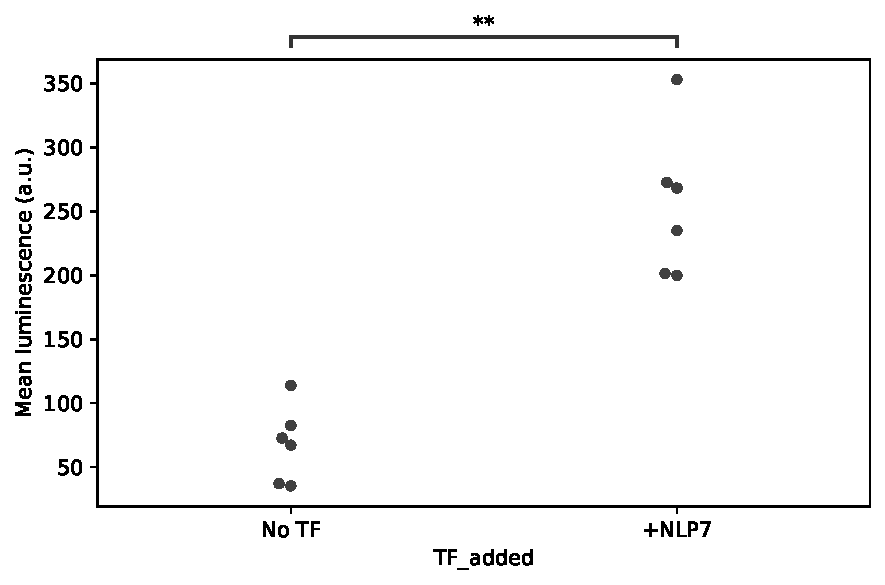
\includegraphics[width=0.60\columnwidth]{luminescence/mar2021_synpromoters/scatter4x[NRE-TATA]+spacing}
		\caption{
			\textbf{Luminescence of the transiently expression 4x[NRE-TATA]+spacing promoter with or without co\hyp{}expression of the NLP7 TF in Arabidopsis leaf protoplasts}
			\SI{1000}{\fmol} of 4x[NRE-TATA]+spacing:LucN plasmid and \SI{500}{\fmol} of delivery calibrator \textit{35S}:LucF used during transformation of protoplasts.
			For TF co\hyp{}expression \SI{1000}{\fmol} of \textit{35S}:NLP7 plasmid DNA was added during transformation.
			\textit{STAP4}, negative control.
			Plants were grown in soil for 3\textendash{}6 weeks before harvesting of protoplasts.
			Significance tested using Mann-Whitney.
			*, \textit{P} \textless{} 0.05.
			\textit{n} = 5\textendash{}6.
			\label{fig:4xnre-tata-spacing}
		}
	\end{center}
\end{figure}

\begin{figure}[hbt!]
	\begin{center}
		\capstart
		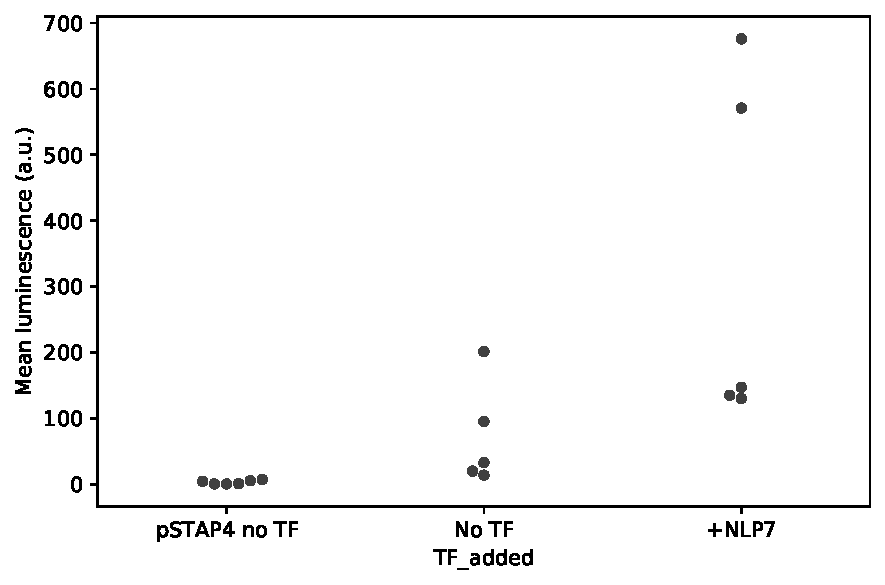
\includegraphics[width=0.60\columnwidth]{luminescence/mar2021_synpromoters/scatter4x[NRE-random]+spacing}
		\caption{
			\textbf{Luminescence of the transiently expression 4x[NRE-random]+spacing promoter with or without co\hyp{}expression of the NLP7 TF in Arabidopsis leaf protoplasts}
			\SI{1000}{\fmol} of 4x[NRE-random]+spacing:LucN plasmid and \SI{500}{\fmol} of delivery calibrator \textit{35S}:LucF used during transformation of protoplasts.
			For TF co\hyp{}expression \SI{1000}{\fmol} of \textit{35S}:NLP7 plasmid DNA was added during transformation.
			\textit{STAP4}, negative control.
			Plants were grown in soil for 3\textendash{}6 weeks before harvesting of protoplasts.
			Significance tested using Mann-Whitney.
			*, \textit{P} \textless{} 0.05.
			\textit{n} = 5\textendash{}6.
			\label{fig:4xnre-random-spacing}
		}
	\end{center}
\end{figure}

\section{Discussion}\label{chapter5:discussion}

The luminescence between different experimental batches was very variable, making it difficult to compare different promoters.
To counteract this, the experiments will be repeated using the same batch of plants to reduce biological variation.

\end{document}